\documentclass[11pt]{article}

\usepackage[review]{acl}

\usepackage{times}
\usepackage{latexsym}
\usepackage[T1]{fontenc}
\usepackage[utf8]{inputenc}
\usepackage{microtype}
\usepackage{inconsolata}
\usepackage{graphicx}
\usepackage{booktabs}
\usepackage{amsmath}
\usepackage{tikz}

\newcounter{algo}
\newcommand{\alghead}[2]{%
  \par\vspace{0.55em}\noindent
  \begin{minipage}{\columnwidth}
  \hrule\vspace{0.4em}
  \refstepcounter{algo}\label{#1}%
  {\small\textbf{Algorithm \thealgo.} #2}\par
  \vspace{0.15em}\hrule\vspace{0.35em}
  \small
}

\definecolor{origlbl}{RGB}{124,115,176}
\definecolor{wmlbl}{RGB}{66,122,196}
\definecolor{cuelight}{RGB}{214,230,248}
\definecolor{skiplight}{RGB}{232,232,236}
\definecolor{revlight}{RGB}{214,240,222}
\definecolor{revedge}{RGB}{32,112,72}
\definecolor{baracw}{RGB}{176,176,184}
\definecolor{barsrc}{RGB}{124,115,176}
\newcommand{\ind}[1]{\hspace*{#1em}}
\newcommand{\codepanel}[3]{%
  \begin{tikzpicture}[baseline=(box.north)]
    \node[draw, line width=0.4pt, inner sep=8pt, outer sep=0pt, anchor=north] (box) {%
      \begin{minipage}[t][4.5cm][t]{0.44\textwidth}
        \scriptsize\ttfamily #3
      \end{minipage}%
    };
    \node[anchor=south east, inner sep=3.5pt, outer sep=0pt, fill=#1, text=white,
          font=\sffamily\scriptsize\bfseries] at (box.south east) {#2};
  \end{tikzpicture}%
}

\title{AcroSplit: Mass-Balanced Red/Green Watermarking for LLM-Generated Code}

\author{Anonymous ACL submission}

\begin{document}
\maketitle
\begin{abstract}

% - to do List: 

% - pseudo code of the algorithm done       
% - diagram or flow of pipeline done
% - add models (minimum 5) for each dataset, add 2 data sets done ~
% - we need to explain the difference btw claude and us done
% - accuracy + token density + pass @ 1 ? ( executed from the first time + pass exam ) done ~
% - change the code in 1\%, 3\% or 5\% and 20\% --> check if the water marking still works or not. --- > robustness test
% - what is the effect on efficiency (tokens/second) : take 2 codes: calculate the token second with and without watermarking done 

% => base 2,370 t/s watermarking 2.381 t/s  almost the same 

We describe AcroSplit, a multi-bit watermark for language-model code generation.
After ordinary sampling filters, every step with at least two surviving candidates is split into green and red lists of similar probability mass; the next message bit selects which list to sample from.
A generation-time $W$-score measures how strongly those splits constrain the sample.
On Qwen3.8-27B, a short list-conversion function carries 20 embedding steps at 0.22 bits per token in executable code, with no comment padding.
Average density is $0.16$--$0.18$ bits/token, about three times ACW and SrcMarker, with $100\%$ bit accuracy.
Relative to classic (unwatermarked) sampling, pass@1 drops $2.1\%$ on InstructHumanEval and $2.8\%$ on MBPP.
On a vLLM serving stack the same protocol holds for smaller code models: Qwen3-8B loses $2.2\%$ relative pass@1 on HumanEval, and DeepSeek-Coder-6.7B-Instruct loses $3.1\%$.
\end{abstract}

\section{How AcroSplit works}
\label{sec:method}

AcroSplit hides a bitstring in the tokens chosen by a language model.
Generation writes the message. Reveal reads it back.
Both procedures share three inputs: the model, the decoding filters, and a secret key.

The message $m$ has length $L$.
Cue $i$ writes bit $m_{i \bmod L}$.
After the last bit, the message repeats from the start.
Figure~\ref{fig:flow} shows one step of each procedure.
Algorithms~\ref{alg:split}--\ref{alg:reveal} state the same steps in full.

\begin{figure*}[t]
\centering
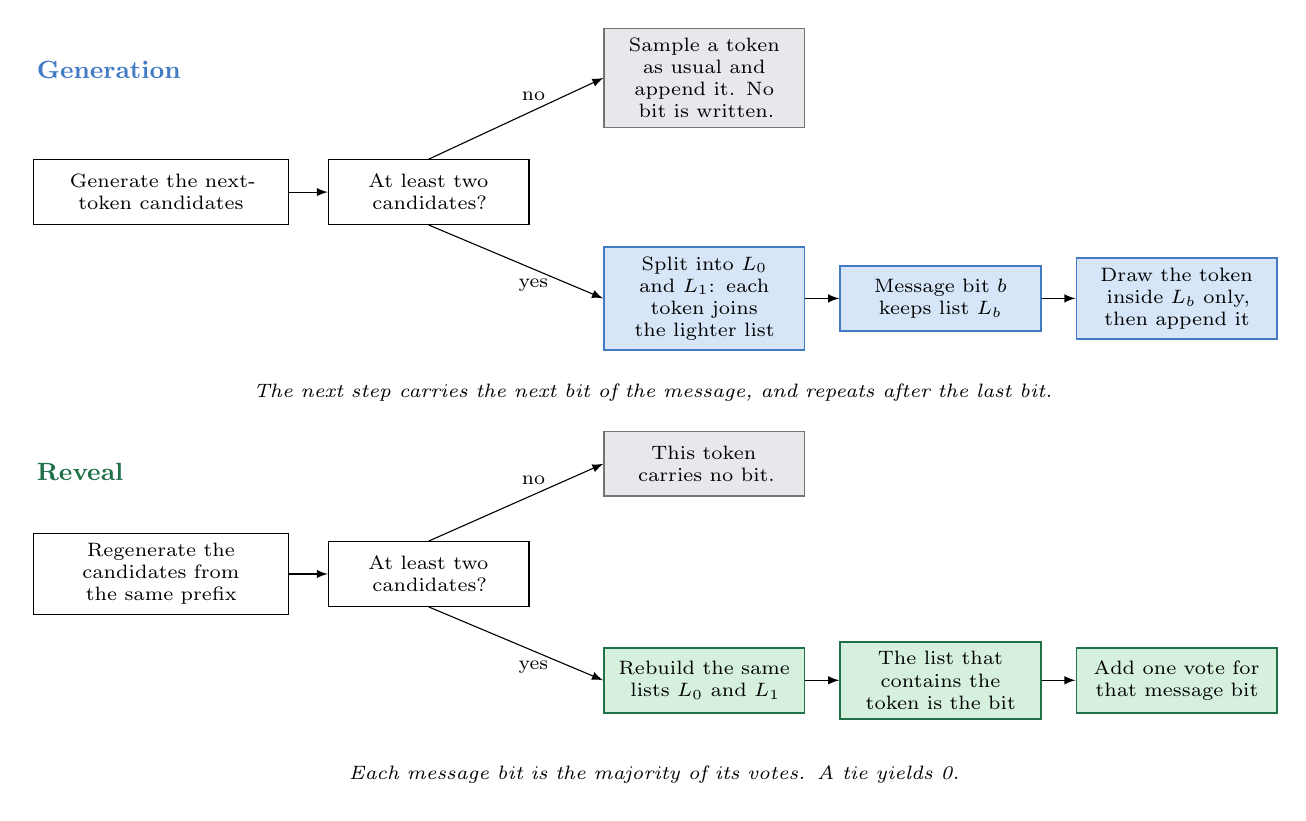
\begin{tikzpicture}[
  font=\scriptsize,
  box/.style={draw, line width=0.45pt, align=center, inner sep=3.5pt,
              minimum height=8.2mm, text width=23mm},
  start/.style={box, text width=30mm, fill=white},
  decide/.style={box, fill=white},
  skip/.style={box, fill=skiplight, draw=black!55},
  cue/.style={box, fill=cuelight, draw=wmlbl, line width=0.7pt},
  rev/.style={box, fill=revlight, draw=revedge, line width=0.7pt},
  note/.style={font=\scriptsize\itshape, align=center, text width=118mm},
  >=latex
]
  \node[font=\small\bfseries, anchor=west, text=wmlbl] at (-1.55,1.55) {Generation};
  \node[start] (gen) at (0.15,0) {Generate the next-token candidates};
  \node[decide] (gate) at (3.55,0) {At least two candidates?};
  \node[skip] (plain) at (7.05,1.45) {Sample a token as usual and append it. No bit is written.};
  \node[cue] (split) at (7.05,-1.35) {Split into $L_0$ and $L_1$: each token joins the lighter list};
  \node[cue] (bit) at (10.05,-1.35) {Message bit $b$ keeps list $L_b$};
  \node[cue] (draw) at (13.05,-1.35) {Draw the token inside $L_b$ only, then append it};

  \draw[->] (gen) -- (gate);
  \draw[->] (gate.north) -- node[above, pos=0.6] {no} (plain.west);
  \draw[->] (gate.south) -- node[below, pos=0.6] {yes} (split.west);
  \draw[->] (split) -- (bit);
  \draw[->] (bit) -- (draw);
  \node[note] at (6.4,-2.55) {The next step carries the next bit of the message, and repeats after the last bit.};

  \node[font=\small\bfseries, anchor=west, text=revedge] at (-1.55,-3.55) {Reveal};
  \node[start] (regen) at (0.15,-4.85) {Regenerate the candidates from the same prefix};
  \node[decide] (rgate) at (3.55,-4.85) {At least two candidates?};
  \node[skip] (rplain) at (7.05,-3.45) {This token carries no bit.};
  \node[rev] (rsplit) at (7.05,-6.2) {Rebuild the same lists $L_0$ and $L_1$};
  \node[rev] (rbit) at (10.05,-6.2) {The list that contains the token is the bit};
  \node[rev] (rvote) at (13.05,-6.2) {Add one vote for that message bit};

  \draw[->] (regen) -- (rgate);
  \draw[->] (rgate.north) -- node[above, pos=0.6] {no} (rplain.west);
  \draw[->] (rgate.south) -- node[below, pos=0.6] {yes} (rsplit.west);
  \draw[->] (rsplit) -- (rbit);
  \draw[->] (rbit) -- (rvote);
  \node[note] at (6.4,-7.4) {Each message bit is the majority of its votes. A tie yields 0.};
\end{tikzpicture}
\caption{One generation step and the matching reveal step.
Gray: the step has fewer than two candidates, so no bit is written or read.
Blue: generation writes the current message bit by sampling inside one list.
Green: reveal reads that bit back from the list which contains the observed token.
$L_0$ is the list for bit 0. $L_1$ is the list for bit 1.}
\label{fig:flow}
\end{figure*}

\subsection{Generation}
\label{sec:gen}

Start from the prompt.
Then, at every step:

\begin{enumerate}
\item \textbf{Filter.} Apply the decoding filters. Keep the surviving candidates in a set $C$. Later draws stay inside $C$.
\item \textbf{Skip.} If $C$ has fewer than two tokens, sample from $C$ in the usual way. This step writes no bit.
\item \textbf{Split.} If $C$ has two or more tokens, split it into two lists, $L_0$ and $L_1$. The rule is Section~\ref{sec:split}.
\item \textbf{Select.} Let $b$ be the current message bit. Keep list $L_b$. Drop the other list.
\item \textbf{Sample.} Draw the next token from $L_b$. Inside that list, probabilities stay proportional to the filtered ones.
\item \textbf{Advance.} Append the token. The next cue carries the next message bit.
\end{enumerate}

\subsection{Split}
\label{sec:split}

Split is fixed by $C$, the key, and $\mathrm{context}(x)$: a short suffix of the prefix already written.
$\mathrm{mass}(L)$ is the total filtered probability of the tokens in $L$.
$L_0$ is the list for bit~$0$. $L_1$ is the list for bit~$1$.

\begin{enumerate}
\item Sort the tokens of $C$ from the most probable to the least probable.
\item Give each token, in that order, to the list whose mass is smaller.
\item If the two masses are equal, hash the key together with $\mathrm{context}(x)$, and use that bit to choose the list. The first token is always a tie.
\end{enumerate}

\subsection{Reveal}
\label{sec:reveal}

Walk the generated tokens, starting again from the prompt.

\begin{enumerate}
\item Recompute $C$ with the same filters on the same prefix.
\item If $C$ has at least two tokens, recompute the same split, and advance the cue index.
\item The list that contains the observed token is the bit recorded for this cue.
\item For each message index, count the votes for $0$ and the votes for $1$.
\item Write $1$ when the votes for $1$ are strictly more numerous. Write $0$ in every other case, including a tie.
\end{enumerate}

\alghead{alg:split}{Split$(C, \mathrm{key}, x)$}
\noindent
sort $C$ by decreasing probability\\
$L_0 \leftarrow \emptyset$,\quad $L_1 \leftarrow \emptyset$\\
$h \leftarrow \mathrm{Hash}(\mathrm{key}, \mathrm{context}(x)) \bmod 2$\\
\textbf{for} each token $t$ in $C$ \textbf{do}\\
\hspace*{1em}\textbf{if} $\mathrm{mass}(L_0) < \mathrm{mass}(L_1)$ \textbf{then} $L_0 \leftarrow L_0 \cup \{t\}$\\
\hspace*{1em}\textbf{else if} $\mathrm{mass}(L_1) < \mathrm{mass}(L_0)$ \textbf{then} $L_1 \leftarrow L_1 \cup \{t\}$\\
\hspace*{1em}\textbf{else} $L_h \leftarrow L_h \cup \{t\}$\\
\textbf{return} $(L_0, L_1)$
\end{minipage}

\alghead{alg:gen}{Generate}
\noindent
$x \leftarrow$ prompt,\quad $i \leftarrow 0$\\
\textbf{while} not done \textbf{do}\\
\hspace*{1em}$C \leftarrow \mathrm{Filter}\bigl(p(\cdot \mid x)\bigr)$\\
\hspace*{1em}\textbf{if} $|C| < 2$ \textbf{then}\\
\hspace*{2em}$t \leftarrow \mathrm{Sample}(C)$\\
\hspace*{1em}\textbf{else}\\
\hspace*{2em}$(L_0, L_1) \leftarrow \mathrm{Split}(C, \mathrm{key}, x)$\\
\hspace*{2em}$b \leftarrow m_{i \bmod L}$\\
\hspace*{2em}$t \leftarrow \mathrm{Sample}(L_b)$ \quad\textit{(relative probabilities)}\\
\hspace*{2em}$i \leftarrow i + 1$\\
\hspace*{1em}append $t$ to $x$\\
\textbf{return} the tokens appended to the prompt
\end{minipage}

\alghead{alg:reveal}{Reveal}
\noindent
$\mathrm{votes}_0[0..L{-}1] \leftarrow 0$,\quad $\mathrm{votes}_1[0..L{-}1] \leftarrow 0$\\
$x \leftarrow$ prompt,\quad $i \leftarrow 0$\\
\textbf{for} each generated token $t$ \textbf{do}\\
\hspace*{1em}$C \leftarrow \mathrm{Filter}\bigl(p(\cdot \mid x)\bigr)$\\
\hspace*{1em}\textbf{if} $|C| \ge 2$ \textbf{then}\\
\hspace*{2em}$(L_0, L_1) \leftarrow \mathrm{Split}(C, \mathrm{key}, x)$\\
\hspace*{2em}$j \leftarrow i \bmod L$\\
\hspace*{2em}\textbf{if} $t \in L_0$ \textbf{then} $\mathrm{votes}_0[j] \leftarrow \mathrm{votes}_0[j] + 1$\\
\hspace*{2em}\textbf{else if} $t \in L_1$ \textbf{then} $\mathrm{votes}_1[j] \leftarrow \mathrm{votes}_1[j] + 1$\\
\hspace*{2em}$i \leftarrow i + 1$\\
\hspace*{1em}append $t$ to $x$\\
\textbf{for} $j = 0$ \textbf{to} $L-1$ \textbf{do}\\
\hspace*{1em}$\hat{m}_j \leftarrow 1$ \textbf{if} $\mathrm{votes}_1[j] > \mathrm{votes}_0[j]$ \textbf{else} $0$\\
\textbf{return} $\hat{m}$
\end{minipage}

\section{Related work}
\label{sec:related}

Work on marking machine-generated text has two largely separate lineages: \emph{logit-level} watermarks that intervene while the model samples, and \emph{post-hoc} watermarks that rewrite a finished artifact.
AcroSplit belongs to the first lineage, but it is built for code, where a usable watermark has to carry a multi-bit payload inside short, executable programs rather than a single detect/not-detect bit in long prose.

The canonical logit-level scheme of \citet{kirchenbauer-etal-2023-watermark} hashes the preceding tokens and partitions the \emph{entire} vocabulary into green and red lists.
Sampling is biased toward green; a $z$-test on green hits then detects the watermark.
That design is strong for long natural-language passages, and later variants make the bias unbiased or distortion-free \citep{zhao2023provable,kuditipudi2024robust} or argue cryptographic undetectability \citep{christ2024undetectable}.
It is a poor fit for code generation on three counts.
First, a random split of the full vocabulary ignores the tiny nucleus that nucleus sampling actually uses, so most of the green list is never a legal next token.
Second, the usual objective is binary detection, not a recoverable message of a few bits.
Third, a heavy green bias can change identifiers and control flow enough to fail unit tests.
AcroSplit keeps the red/green vocabulary of that literature, but it splits only the filtered candidate set $C$, balances the two lists by probability mass rather than by a hash of token ids, and spends each cue on the next bit of a repeating payload.
The mass balance is why either bit remains a high-probability continuation, which is the quantity that pass@1 measures.

A second line of work watermarks \emph{source code after it has been written}.
ACW \citep{li2024acw} and SrcMarker \citep{yang2024srcmarker} encode bits by applying semantics-preserving transforms and identifier rewrites to a finished program.
Those methods do not need the generator, so they apply to human code as well as to model output.
The channel, however, is sparse: on HumanEval and MBPP snippets the static capacity is about one bit every 16--18 tokens (Section~\ref{sec:density}), and recovery is imperfect ($97.2\%$ and $97.3\%$ BitAcc) because a transform that already matches the original is scored as an error.
AcroSplit cannot mark a program that was not sampled under the key, but it does not wait for a finished AST either.
Every splittable decoding step is a cue, density is about three times higher on Qwen3.8-27B, and reveal replays the same keyed split, so cue-level BitAcc is $100\%$ whenever the split ran.

The evaluation of code generators themselves \citep{chen2021evaluating,austin2021program} is the right testbed for this distinction.
A watermark that survives only as comments, or that drops pass@1 by a large relative margin, is not a watermark on \emph{code generation}.
Section~\ref{sec:results} therefore reports functional pass@1 against matched classic sampling, not only retrieval.

\section{Watermarking score}
\label{sec:wscore}

The lists hold only candidates that survived filtering, and the split keeps their masses close.
A random green/red hash partitions the full vocabulary, with no mass balance.
The two lists are rarely perfectly balanced.
Write $m_t$ for the total filtered probability of the list selected at cue $t$, measured \emph{before} masking.
A bit that picks the heavy side yields $m_t \gg 0.5$; a bit that picks the light side yields a small $m_t$.
Unwatermarked text tends to occupy the heavier list (occupied mass around $0.6$--$0.63$ in our checks).
A watermarked sample, because the bit chooses independently of mass, sits closer to one half on average.

Hide always forces a hit on the chosen list, so a raw green-hit count is not informative at generation time.
We instead accumulate a soft $z$-score from the chosen masses alone:
\begin{equation}
  W \;=\;
  \frac{\sum_t (1 - m_t)}
       {\sqrt{\sum_t m_t\,(1 - m_t)}}\,.
  \label{eq:wscore}
\end{equation}
Each cue behaves like a Bernoulli trial that always succeeds while the null success probability is $m_t$.
Sampling the light list (small $m_t$) contributes more; many cues near $m_t \approx 0.5$ still drive $W$ upward.
A large positive $W$ on a generated sample means the sequence was produced under the watermark constraint over many unbalanced splits.
It is a generation-time strength signal, not a stand-alone keyless detector.

\section{Results}
\label{sec:results}

The following measurements share the same protocol: matched classic sampling versus AcroSplit, same prompts, same filters.
We report an example, token density and BitAcc against post-hoc code watermarks, generation throughput, then pass@1 on Qwen3.8-27B and on additional models served with vLLM.

\subsection{Hiding bits in short programs}
\label{sec:example}

Because every splittable nucleus step carries a bit, short functions can still host many cues even when the model writes ordinary executable statements rather than comments.
Figure~\ref{fig:sidebyside} shows MBPP task~117, \texttt{list\_to\_float}: recursively (classic) or by a list comprehension (AcroSplit), convert nested string fields to floats.
Both completions are comment-free.
AcroSplit uses $20$ embedding steps (density $0.22$) and recovers the $4$-bit payload \texttt{0100} in full.
The two programs differ in identifiers, control structure, and \texttt{str} vs.\ \texttt{repr}---the kind of variation the mass-balanced split is meant to harvest.

\begin{figure*}[t]
\centering
\codepanel{origlbl}{Original code}{%
def list\_to\_float(lst):\\
\ind{1}def convert\_to\_float(item):\\
\ind{2}if isinstance(item, (list, tuple)):\\
\ind{3}return type(item)(convert\_to\_float(\\
\ind{4}subitem) for subitem in item)\\
\ind{2}try:\\
\ind{3}return float(item)\\
\ind{2}except (ValueError, TypeError):\\
\ind{3}return item\\
\ind{1}converted = convert\_to\_float(lst)\\
\ind{1}return str(converted)%
}%
\hfill
\codepanel{wmlbl}{Watermarked code}{%
def list\_to\_float(lst):\\
\ind{1}def convert\_to\_float(item):\\
\ind{2}try:\\
\ind{3}return float(item)\\
\ind{2}except (ValueError, TypeError):\\
\ind{3}return item\\
\ind{1}result = [\\
\ind{2}tuple(convert\_to\_float(x) for x in inner)\\
\ind{2}if isinstance(inner, (tuple, list))\\
\ind{2}else convert\_to\_float(inner)\\
\ind{2}for inner in lst\\
\ind{1}]\\
\ind{1}return repr(result)%
}%
\caption{Same MBPP task, both programs pass the unit tests.
Left: classic sampling (original).
Right: AcroSplit (watermarked; $20$ cues).
The $4$-bit message is retrieved by majority vote over those cues.}
\label{fig:sidebyside}
\end{figure*}

\subsection{Token density}
\label{sec:density}

Token density is hideable bits per token.
ACW \citep{li2024acw} and SrcMarker \citep{yang2024srcmarker} post-process a finished program: each applicable transform (or name rewrite) is one bit.
On 539 HumanEval and MBPP snippets that yields $0.056$ and $0.061$ bits/token---about one bit every 16--18 tokens.
AcroSplit instead spends a bit at every splittable decoding step.
On Qwen3.8-27B that is $0.159$ bits/token on InstructHumanEval and $0.180$ on MBPP (Figure~\ref{fig:density}), roughly $3\times$ denser.

\begin{figure}[t]
\centering
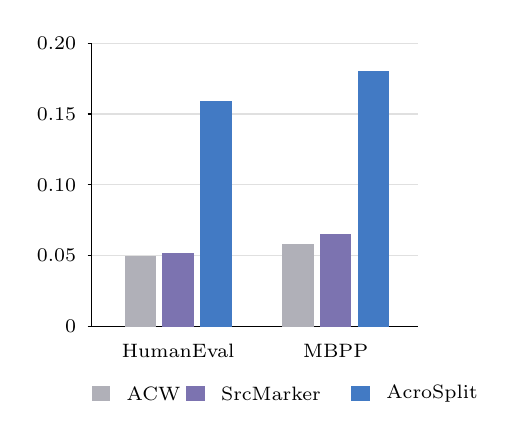
\begin{tikzpicture}[x=1cm,y=1cm,font=\scriptsize]
  \foreach \yy in {0,0.9,1.8,2.7,3.6}
    \draw[black!12] (0,\yy) -- (4.15,\yy);
  \draw (0,0) -- (0,3.6);
  \draw (0,0) -- (4.15,0);
  \foreach \lab/\yy in {0/0, 0.05/0.9, 0.10/1.8, 0.15/2.7, 0.20/3.6}{
    \draw (-1.4pt,\yy) -- (0,\yy);
    \node[anchor=east] at (-2pt,\yy) {\lab};
  }
  \fill[baracw] (0.42,0) rectangle (0.82,0.900);
  \fill[barsrc] (0.90,0) rectangle (1.30,0.936);
  \fill[wmlbl]  (1.38,0) rectangle (1.78,2.862);
  \node[anchor=north] at (1.10,-0.10) {HumanEval};
  \fill[baracw] (2.42,0) rectangle (2.82,1.044);
  \fill[barsrc] (2.90,0) rectangle (3.30,1.170);
  \fill[wmlbl]  (3.38,0) rectangle (3.78,3.240);
  \node[anchor=north] at (3.10,-0.10) {MBPP};
  \fill[baracw] (0.00,-0.95) rectangle ++(0.24,0.20);
  \node[anchor=west] at (0.32,-0.85) {ACW};
  \fill[barsrc] (1.20,-0.95) rectangle ++(0.24,0.20);
  \node[anchor=west] at (1.52,-0.85) {SrcMarker};
  \fill[wmlbl]  (3.30,-0.95) rectangle ++(0.24,0.20);
  \node[anchor=west] at (3.62,-0.85) {AcroSplit};
\end{tikzpicture}
\caption{Bits per token.}
\label{fig:density}
\end{figure}

Bit accuracy (BitAcc) is the fraction of embedded bits recovered in the clear.
ACW checks whether each transform was applied; a transform that already matches by chance is an error, so BitAcc averages $97.2\%$ \citep{li2024acw}.
SrcMarker learns which transforms and names to use; BitAcc is $97.3\%$ on Java \citep{yang2024srcmarker}.
AcroSplit reveal replays the same keyed split.
The replay is deterministic, so the votes for one message index agree, and every cue is recovered: BitAcc is $100\%$.

\begin{table}[t]
\centering
\small
\begin{tabular}{@{}lc@{}}
\toprule
 & BitAcc (\%) \\
\midrule
ACW & $97.2$ \\
SrcMarker & $97.3$ \\
AcroSplit & $100$ \\
\bottomrule
\end{tabular}
\caption{BitAcc.
ACW: mean over 4-bit encodings, uncorrected \citep{li2024acw}.
SrcMarker: $SrcMarker_{\mathrm{TE}}$ on CSN-Java \citep{yang2024srcmarker}.
AcroSplit: cue-level recovery on Qwen3.8-27B.}
\label{tab:bitacc}
\end{table}

\subsection{Generation throughput}
\label{sec:overhead}

AcroSplit is applied after the filtered next-token distribution is already known.
The extra work is a partition of that shortlist and a draw from one side.
We measure end-to-end speed in tokens per second.

Classic sampling produces $2.381$ tokens/s and AcroSplit $2.370$ tokens/s (Table~\ref{tab:overhead}).
The two rates match.

\begin{table}[t]
\centering
\small
\begin{tabular}{@{}lcc@{}}
\toprule
 & Classic & AcroSplit \\
\midrule
Tokens/s & $2.381$ & $2.370$ \\
\bottomrule
\end{tabular}
\caption{Generation throughput (tokens/s).}
\label{tab:overhead}
\end{table}

\subsection{Pass@1 versus classic sampling}
\label{sec:pass}

Table~\ref{tab:pass} compares functional pass@1 of classic sampling against AcroSplit.
The runs share the prompts and the decoding filters: temperature, top-$k$, and nucleus.
Because the split balances probability mass, either message bit stays a plausible continuation under the model.
Relative change is $(w-u)/u$ against the matched classic run.

On Qwen3.8-27B, AcroSplit loses $1.8$ points ($2.1\%$ relative) on InstructHumanEval and $2.0$ points ($2.8\%$ relative) on full MBPP.
Most classic-passing tasks still pass with the watermark.
Density and cue-level BitAcc on that model are those of Section~\ref{sec:density}.

\subsection{Additional models on vLLM}
\label{sec:vllm}

The Qwen3.8-27B numbers use an OpenAI-compatible completions API that returns the top-$20$ log-probabilities at every step; AcroSplit then splits that shortlist on the client.
The same protocol runs on other vLLM endpoints without changing the split.

\paragraph{Qwen3-8B, HumanEval.}
We generate classic and AcroSplit completions for all $164$ HumanEval tasks ($T{=}0.9$, nucleus $0.9$, top-$20$).
Classic pass@1 is $82.3\%$ and AcroSplit $80.5\%$ (relative $\Delta=-2.2\%$; Table~\ref{tab:pass}).
Mean density is $0.145$ bits/token.
Reveal replays the same keyed split, so BitAcc is $100\%$.
The drop in pass@1 is a utility cost of the split, not a failure of reveal.

\paragraph{DeepSeek-Coder-6.7B-Instruct, HumanEval.}
The same HumanEval suite on a vLLM DeepSeek-Coder-6.7B-Instruct endpoint yields classic pass@1 $67.1\%$ and AcroSplit $65.0\%$ (relative $\Delta=-3.1\%$), density $0.138$ bits/token, and BitAcc $100\%$.

In both cases the extra decision work after the top-$20$ list is already available remains sub-millisecond, consistent with Section~\ref{sec:overhead}: serving, not the split, dominates wall time.

\begin{table*}[t]
\centering
\small
\begin{tabular}{@{}llrrrrr@{}}
\toprule
Model & Dataset & Classic & AcroSplit & Rel.\ $\Delta$ & Dens. & BitAcc \\
\midrule
Qwen3.8-27B & InstructHumanEval & $86.6$ & $84.8$ & $-2.1\%$ & $0.159$ & $100$ \\
Qwen3.8-27B & MBPP & $71.0$ & $69.0$ & $-2.8\%$ & $0.180$ & $100$ \\
Qwen3-8B & HumanEval & $82.3$ & $80.5$ & $-2.2\%$ & $0.145$ & $100$ \\
DeepSeek-Coder-6.7B & HumanEval & $67.1$ & $65.0$ & $-3.1\%$ & $0.138$ & $100$ \\
\bottomrule
\end{tabular}
\caption{Pass@1 (\%), mean density (bits/token), and cue-level BitAcc (\%).
InstructHumanEval and HumanEval $n{=}164$; MBPP is the full test set.
BitAcc is $100\%$ because reveal replays the same keyed split.
Rel.\ $\Delta$ is $(w-u)/u$ vs.\ classic sampling.}
\label{tab:pass}
\end{table*}

\bibliography{custom}

\end{document}
